\chapter{Multi User Interaktion}
\label{ch:Multi_User_Interaktion}

\section{Realisierung}
Mit dem Projekt und den Erkenntnissen des Single-User Prototypen begann die Erstellung eines Multi-User tauglichen Prototypen.

\subsection{Multi User}
Um die Applikation Multi-User tauglich zu machen, wurde die Photon-Engine verwendet (\cite{noauthor_photon_2019}). Diese Engine stellt ein Unity-Asset zur Verfügung mit verschiedenen Beispielen wie die Engine einzusetzen ist. \\

\noindent Auf der Webseite von Photon kann nach einem erfolgreichen Login eine neue Applikation erstellt werden. Für den Multi-User Prototyp wurde eine Realtime-Applikation erstellt mit bis zu 20 gleichzeitigen Benutzern. Soll eine Applikation mit mehr als 20 gleichzeitigen Nutzern erstellt werden, wird dies kostenpflichtig. Nach dem erstellen kann die erhaltene App ID, zu sehen in Abbildung \ref{fig:photon_dashboard}, in Unity verwendet werden.

\begin{figure}[h!]
	\centering
	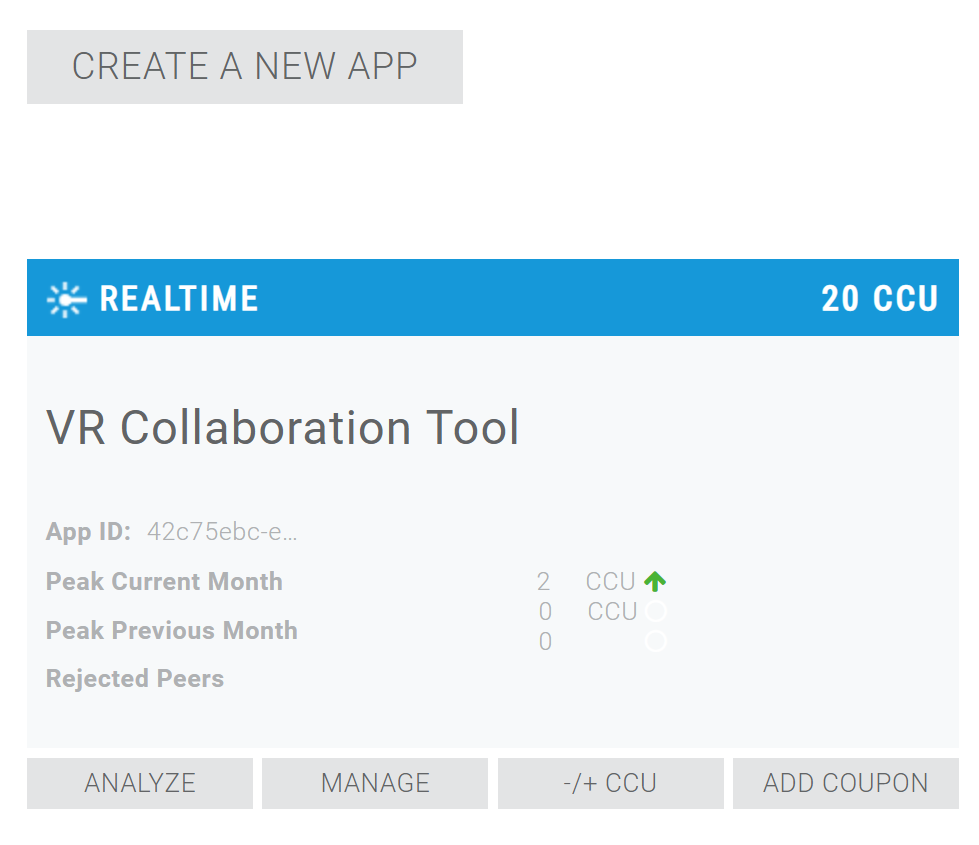
\includegraphics[keepaspectratio,width=0.4\linewidth]{img/Photon_Dashboard.PNG}
	\caption{Photon Dashboard}
	\label{fig:photon_dashboard}
\end{figure} 

Mit der App ID kann Unity sich nun auf die Applikation verbinden. Die erste Instanz, welche sich verbindet wird automatisch als Master deklariert. Um nun mit anderen Instanzen kommunizieren zu können, müssen diese sich mit einen virtuellen Raum verbinden. Sobald sich beide im gleichen Raum befinden, kann die Kommunikation beginnen.\\
Jeglichen Objekten, welche nun untereinander synchronisiert werden sollen, muss die Komponente Photon View hinzugefügt werden. Diese besitzt die folgenden Parameter:
\begin{itemize} [itemsep=1pt]
	\item Owner: Der aktuelle Besitzer der Objekts
	\item View ID: Eindeutige Identität des Objektes
	\item Observed Components: Welche Komponenten des Objektes mit den anderen Instanzen synchronisiert werden soll.
\end{itemize}

Für die Synchronisation vieler standardmässigen Unity-Komponenten stellt die Photon-Engine schon Komponenten zur Verfügung. Eine dieser Komponenten, die Photon Transform View, wurde im Prototyp verwendet, um die Position und die Rotation des Objektes zu synchronisieren. Somit werden diese beiden Eigenschaften mit allen Instanzen synchronisiert, welche nicht Besitzer des Objektes sind. Es ist aber nicht möglich als Nicht-Besitzer ein Objekt zu bewegen. \\
Die Master-Instanz wird bei der Initialisierung Besitzer von allen Objekten, welche eine Photon View besitzen. Um als Nicht-Master-Instanz nun ein Objekt bewegen zu können, stellt die Photon-Engine die Funktion \textit{RequestOwnership()} zur Verfügung. Diese Funktion macht die Instanz zum neuen Besitzer der Photon View, welche die Funktion aufgerufen hat. Somit kann nun die Nicht-Master-Instanz das Bauteil bewegen und alle anderen Instanzen sehen diese Bewegung. \\

\noindent Da die Bauteile im Prototyp einen Rigidbody angehängt haben, muss auch dieser synchronisiert werden. Die Photon-Engine stellt aber für die Synchronisation eines Rigidbody keine Komponenten zur Verfügung. Sie stellt aber die Methode \textit{OnPhotonSerializeView(PhotonStream stream, PhotonMessageInfo info)} zur Verfügung, mit welcher eigene Attribute zwischen den Instanzen synchronisiert werden können. Die Methode wird standardmässig 10 mal in der Sekunde aufgerufen, kann aber in den Einstellungen angepasst werden. Nachfolgend ein Ausschnitt wie der Aufbau dieser Methode aussehen sollte.

\begin{algorithm}
	\KwIn{PhotonStream, PhotonMessageInfo}
	\eIf{Falls die aktuelle Instanz auf den Stream schreibt} {
		Schreibe alle Informationen des Rigidbody auf den Stream\;
		Schreibe weitere Attribute auf den Stream\;
	}{
		Lese die Informationen aus dem Stream und speichere diese in den Rigidbody\;
		Lese die weiteren Attribute aus dem Stream\;	
	}
\end{algorithm}

Eine Instanz kann nur dann auf den Stream schreiben, wenn sie in besitzt der Photon View ist. Die Komponente Photon Transform View funktioniert sehr ähnlich wie der beschriebene Pseudocode.

\subsection{Avatar-Repräsentation in der virtuellen Umgebung}

\subsection{Kommunikation zwischen den Benutzern}

%TODO: Website mit API-Key

\subsection{Gleichzeitige Interaktion am selben Objekt}

\section{Evaluation}

\section{Schlussfolgerung}

\section{Systemarchitektur}

\section{Klassendiagramm}